\section{Emotional Competence and Wisdom: Lifespan Developmental Perspectives} \shorttitle{Adult Development of Socio-Emotional Competences
}

One-sided views of aging and old age still exist in our society as well as in scientific circles. On the one hand, old age has been portrayed as a period of disengagement, social isolation, cognitive inflexibility, and physical decline. On the other, many people, especially older people themselves have described old age as a productive life period full of energy, new and inspiring experiences, and gratifying moments. Lifespan developmental researchers have argued that images of old age and aging that are either too negative or too positive run the risk of being dysfunctional. Overly pessimistic views lead to disregard for the possibility that many older people have great potential and could provide valuable contributions to societal life. Illusory positive views put unnecessary pressure on those older people who have experienced age-related losses and hinder social policies aimed at improving their living situations.

 Adopting a lifespan developmental approach, the overarching goal of our research has been to contribute to a balanced picture of aging and old age that encompasses loss, continuity, and growth. According to lifespan developmental psychology, the complexity of developmental processes during adulthood can be described on at least four levels. First, development is multidirectional. During the same developmental period, some realms of functioning decline, while others remain stable, and yet others increase. Second, development is multifunctional. Depending on the criteria that are being considered (e.g., subjective vs. objective or long-term vs. short-term), the same developmental outcome can be considered as gain or loss. Third, development varies among individuals and various social, educational, and ethnic groups. Depending on the individual's personal and social resources, the same realm of functioning may decline, increase, or remain unchanged during adulthood and old age. Fourth, people do not exist in isolation, but are embedded in historical, cultural, and social contexts that provide both developmental opportunities and constraints.

 Two realms of functioning, which are at the center of our research, are ideally suited to demonstrate the complexity of the aging process on the four levels described above. These are emotional competence and wisdom. The primary purpose of our research is to demonstrate that the development of emotional competence and wisdom is differential. That is, it evinces multidirectionality, varies among individuals, is contextually-bound, and simultaneously involves gains and losses. This differentiated view of development helps expand and supplement more traditional conceptualizations that have emphasized universal and general developmental processes and equate development with growth. 

\subsection{Emotional Competence}

\index{Kunzmann, Ute}

\paragraph{Research Team}
Ute Kunzmann (Professor), David Richter (Doctoral Fellow).

 The concept of emotional competence has received widespread attention in several psychological disciplines and various definitions have recently been suggested, differing in terms of content and breadth. Ute Kunzmann and her collaborators have considered emotional competence as a multidimensional concept that covers several distinct facets, including the capacity to spontaneously react to emotion-arousing events with the appropriate emotion, the ability to voluntarily regulate one's own emotions, and the ability to accurately detect other's emotions.
 
 Keeping in mind that people's subjective evaluations of what they can do are sometimes not accurate reflections of their ``objective'' competencies, Ute Kunzmann has begun to design and conduct well-controlled experimental studies in which emotions and emotional abilities can be observed in vivo. In these studies, adults of different ages are exposed to the same emotionally challenging tasks and their subsequent cognitive and emotional reactions are observed objectively. Evidence from this research is meant to supplement the findings from studies employing self-report questionnaires and performance-based tests of emotional competence. 

Findings from the Kunzmann's and her collaborators' laboratories strongly support the general propositions of life-span developmental psychology described above. For example, there is robust evidence for multidirectionality in the realm of emotional reactivity. Whereas autonomic reactions seem to decline with age, subjective reactions remain stable. Furthermore, this pattern of age differences is not fixed but at least partly determined by contextual factors such as the age-relevance of the emotion-arousing event. When being exposed to emotion-evoking themes that are particularly salient in old age, older adult's reactions are greater or just as large than those of young adults - even on the level of autonomic activity.  

Ute Kunzmann and her collaborators at the University of California, Berkeley also provided first performance-based evidence that the ability to regulate one's own emotional reactions on command remains unchanged over adulthood and old age. This evidence refers to one particular form of emotion regulation, that is, the ability to voluntarily up- and down regulate one's facial expressions. Given that emotion regulation comprises multiple forms, the question arises of whether the current evidence can be generalized to other forms of emotion regulation (e.g., the ability to re-evaluate negative experiences so that they become less threatening to the self). An experimental study that Ute Kunzmann designed together with Prof. Fredda Blanchard Fields at the Georgia Institute of Technology, Atlanta will begin to address this question in the near future.

\null
\textbf{Research Highlights 2006}

\textit{Study on Empathic Accuracy: First Results}

 Our research activities during the last months have focused on yet another emotional ability, namely, the \textit{ability to accurately perceive other people's emotions} (i.e., empathic accuracy). As is true for so many resource-demanding and effortful functions, the empirical evidence generally suggests that young adults outperform older adults in tasks assessing this ability. However, a serious limitation of the typical paradigm used to study age differences in empathic accuracy is its lack of ecological validity. Participants are typically asked to recognize emotions from still photographs of faces, which provide very little information about the evaluated persons. Moreover, emotions are typically posed rather than truly experienced. Studying emotion recognition via tasks that are less stripped down in terms of familiarity and meaningfulness might yield a very different picture about age differences in this ability.  

 To test this proposal, Ute Kunzmann and David Richter conducted a study with more contextualized empathic accuracy tasks in our lab. Instead of presenting to young and old adults photographs of people posing prototypical emotions, they presented eight short film clips each dealing with a person as he or she was talking about an emotionally engaging issue. The to be evaluated people experienced real and authentic emotions while talking. To study the role of motivational factors, the age relevance of the topics the videotaped people were talking about was manipulated. One topic was of particular relevance to older people and dealt with age-related losses. A second topic was of particular relevance to young people and dealt with an adventurous and risky life transition. 

 As can be seen in Figure \ref{fig1:profUteKunzmann}, the age-related decline in emotion recognition found in earlier studies was only evident in situations that were of minor relevance to older people. In contrast, there was no age difference in performance level when the task was to accurately evaluate the emotions of a person who talked about a topic that was particularly relevant in old age. Two conclusions from this work are that age-related decline in resource-demanding processes may be limited to tasks and contexts that are of little relevance to older people and that motivational factors can offset age-related deficits. Ute Kunzmann and David Richter organized a symposium with the title ``lifespan development of emotions and emotional competencies'' at the 45th Congress of the German Society for Psychology in September 2006 in the context of which they presented their latest findings. In addition, they are about to submit a grant proposal to the German Research Foundation that will allow them to test additional moderators of the relationship between age and empathic accuracy.

\begin{figure}[htb]
  \begin{center}
    \resizebox{0.5\textwidth}{!}{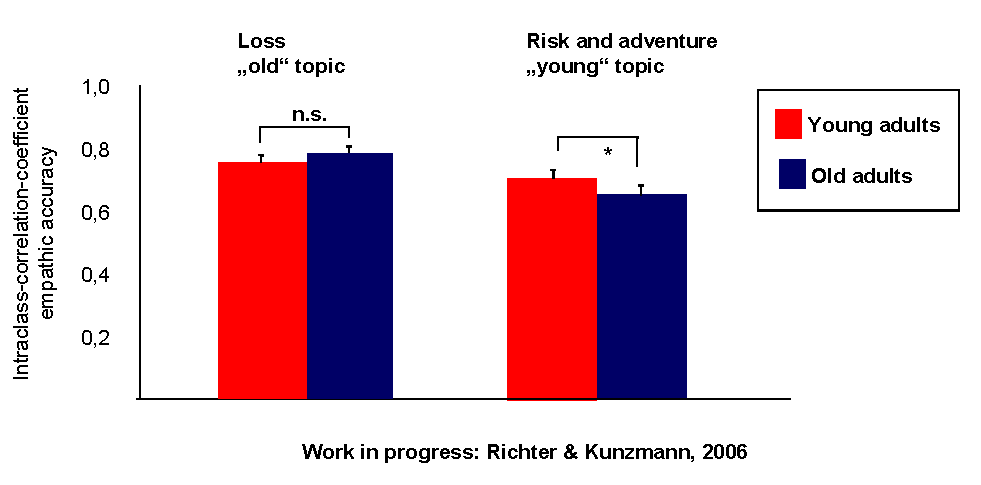
\includegraphics{profUteKunzmann-fig1}}
    \caption{Age differences in empathic accuracy: Age relevance matters.}
    \label{fig1:profUteKunzmann}
  \end{center}
\end{figure}



\textit{Research Network from the German Research Foundation}

 Another research highlight of the last year was a first meeting of a research network funded by the German Research Foundation (faculty member: Ute Kunzmann; student member: David Richter). The network consists of German researchers who study the differential and general development of emotions and emotional competencies. The network members (1/3 faculty and 2/3 graduate students) will hold two meetings per year for a period of three years. The meetings will be designed (a) to facilitate exchange of ideas and expertise, (b) to discuss research with invited internationally distinguished emotion researchers (two guests per meeting), and (c) to develop plans for future collaborative research projects.

\paragraph{Collaborations}
\begin{itemize}
\item Georgia Institute of Technology, Atlanta, USA \\ Prof. Fredda H. Blanchard-Fields, PhD
\item University of California, Berkeley, USA \\ Prof. Robert W. Levenson, PhD
\item University of Geneva, Geneva, CH \\ Prof. Gisela Labouvie-Vief, PhD
\end{itemize}

\begin{bibunit}[apalike]
\nocite{*}
\putbib[profUteKuzmann1]
\end{bibunit}



\paragraph{Grants}

\begin{itemize}
	\item BMBF (PI: JCLL). U. Kunzmann, U.M. Staudinger: subproject ``Images of Aging'' within the joint research project ``Effects of Matches/Mismatches between Aspects of Human and Social Capital, Corporate Strategy and Work Organization on the Physical and Mental Well-Being of Employees''. 
\end{itemize}



\subsection{Emotions in Art}

\index{Kuzmann, Ute}

\paragraph{Research Team}
Ute Kunzmann (Professor), Caroline Schuster Cordone (Doctoral Candidate (University of Fribourgh, Switzerland).

 This project deals with a research topic that transcends disciplinary boundaries. Funded by the International Max Planck Research Network on Aging in November 2006, the central goal of the project is to contribute to a better understanding of the ways in which emotions are expressed in paintings by joining forces and combining art historical and psychological approaches. Ute Kunzmann and her art historical colleague Caroline Schuster Cordone pan to compare art historical and psychological interpretations of the emotional expressions of young and old figures as they are depicted in paintings spanning several epochs. 

 The two psychological approaches to interpreting emotional expressions in paintings are illustrated through a self-portrait of Rembrandt in Figures \ref{fig2:profUteKunzmann} and \ref{fig3:profUteKunzmann}. As can be seen in Figure \ref{fig2:profUteKunzmann}, the expert-based approach to describing emotional expressions in paintings will be based on Paul Ekman's Facial Action Coding System. According to this system, Rembrandt expresses moderate happiness blended with another emotion, most likely slight surprise. 

\begin{figure}[htb]
  \begin{center}
    \resizebox{0.5\textwidth}{!}{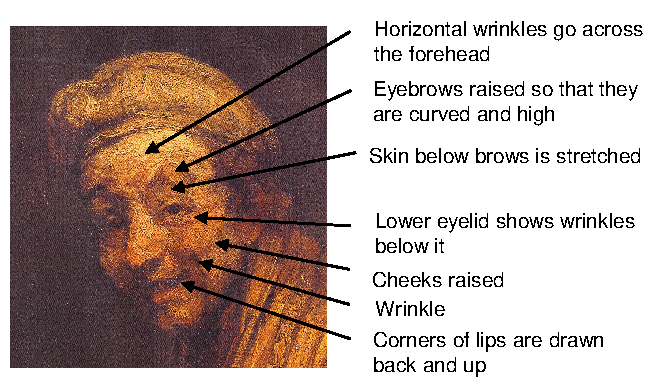
\includegraphics{profUteKunzmann-fig2}}
    \caption{Emotional expressions in paintings: An expert-based approach}
    \label{fig2:profUteKunzmann}
  \end{center}
\end{figure}

The consensus-based approach to describing emotional expressions in paintings is illustrated through the same self-portrait of Rembrandt (see Figure \ref{fig3:profUteKunzmann}). 

\begin{figure}[htb]
  \begin{center}
    \resizebox{0.4\textwidth}{!}{\includegraphics{profUteKunzmann-fig3}}
    \caption{Emotional expressions in paintings: A consensus-based approach.}
    \label{fig3:profUteKunzmann}
  \end{center}
\end{figure}

This approach is based on laypeople's intuitive understanding of emotions. In a pilot study, young and old laypeople were asked to evaluate the painting in terms of which emotions are depicted. Results supported the expert-based codings and revealed that Rembrandt expresses moderate happiness blended with slight surprise. However, there was also high consensus among laypeople that Rembrandt was mischievous and somewhat ironic. The latter two affective states are not part of Ekman's coding system.

\paragraph{Collaborations}
\begin{itemize}
\item University of Fribourg \\ Caroline Schuster Cordone
\end{itemize}

\paragraph{Grants}

\begin{itemize}
\item Maxnet Aging, Max Planck Society (Start 2007). (PI : U. Kunzmann): Expression of emotions in Art: Art Historical and Psychological Perspectives.
\end{itemize}

\subsection{Wisdom}

\index{Kuzmann, Ute}

\paragraph{Research Team}
Ute Kunzmann (Professor), David Richter (Doctoral Fellow).

 Although the psychology of wisdom is a relatively new field, several promising theoretical and operational definitions of wisdom have been developed during the last years (for reviews see Kunzmann, in press; Kunzmann \& Baltes, in press; Kunzmann \& Stange, in press). Our own work has been based on the Berlin wisdom paradigm that defines wisdom as expert knowledge about fundamental problems related to the meaning and conduct of life. In this paradigm, participants think aloud about difficult and uncertain life problems. Trained raters evaluate these think-aloud protocols according to five criteria indicating wisdom. The three core criteria are: (1) value relativism and tolerance, (2) awareness and management of uncertainty and (3) lifespan contextualism. 

 The goal of our research program has been to study the social and emotional dynamics of wisdom-related knowledge in the context of correlational field studies and experimental work. With this goal we intend to produce evidence that highlights the gains that come with the acquisition of wisdom-related knowledge during ontogenesis and especially the difference that this type of knowledge makes in adults' actual social and emotional behavior.

\null
\textbf{Research Highlights 2006}

 During the last year, Ute Kunzmann completed several publications dealing with the motivational, affective and social dynamics of wisdom-related knowledge. As to the social-emotional dynamics of wisdom-related knowledge, her experimental work suggests that people with high levels of wisdom-related knowledge tend to experience greater empathic sadness when being together with another person in need than people with low levels of wisdom-related knowledge. There is also evidence for a link between wisdom-related knowledge and empathic accuracy: wisdom-related knowledge seems to help people perceive other people's emotions accurately. 

 In her field studies Ute Kunzmann and her collaborators have demonstrated that the values and behaviors of people with high levels of wisdom-related knowledge indicate a striving for a good life in the sense of early Greek philosophy. One aspect of a good life in the early Greek tradition refers to the balancing of personal and common interests. A second aspect refers to the preference for personal growth and self-actualization -- even if this preference opposes happiness in a hedonistic and materialistic sense. Together the evidence from Ute Kunzmann and her collaborators strongly supports the general hypothesis that wisdom-related knowledge makes a difference in people's daily life and has important motivational and social functions for one's own and others' development. 

\newpage
\paragraph{Collaborations}
\begin{itemize}
\item Georgia Institute of Technology, Atlanta, USA  \\ Dr. Antje Stange
\item Tufts University, Medford, USA \\ Prof. Robert J. Sternberg, PhD
\end{itemize}

\enlargethispage*{0.2cm}

\begin{bibunit}[apalike]
\nocite{*}
\putbib[profUteKunzmann3]
\end{bibunit}

\subsection{Awards, Fellowships}
\begin{itemize}
\item Junior Fellow of the Max Planck International Research Network on Aging. 
\end{itemize}

\subsection{Other Professional Activities}  

\begin{itemize}
\item Consultant on methods to assess physiological and behavioral aspects of emotion with NIH Project; PI: Prof. Dr. Blanchard-Fields, Georgia Institute of Technology, Atlanta.
\item Faculty member of the research network ``Differential and General Development of Emotion'' funded by the German Research Foundation (HO 1718/5-1).
\end{itemize}

\textit{Editorial Board Membership}

\begin{itemize}
\item Psychology and Aging.
\end{itemize}

\vspace{0.5ex}
\textit{Ad-hoc Reviews}

\begin{itemize}
\item Swiss National Science Foundation.
\end{itemize} 
